%%%%%%%%%%%%%%%%%%%%%%%%%%%%%%%%%%%%%%%%%%%
%%%%%%  STYLE 22
%%%%%%%%%%%%%%%%%%%%%%%%%%%%%%%%%%%%%%%%%%%
\restoregeometry

\newgeometry{left=4.5cm,right=2.5cm, marginparsep=15pt, marginparwidth=4.2cm,top=2cm,%
reversemarginpar}

\cxset{style22/.style={
 name={},
 numbering=none,
 number font-size=\Large,
 number font-family=\rmfamily,
 number font-weight=\bfseries,
 number before={},
 number after={},
 number position=rightname,
 chapter font-family=\sffamily,
 chapter font-weight=\normalfont,
 chapter font-size=\Large,
 chapter before={\vspace*{-10pt}},
 chapter after={},
 chapter color={black!90},
 number color=\color{black!90},
 title beforeskip={\raggedleft},
 title afterskip={\vspace{70pt}},
 title before=\hspace*{-2cm},
 title after={},
 title font-family=\sffamily,
 title font-color=\color{black},
 title font-weight=\bfseries,
 title font-size=\huge,
 section numbering=none,
 section font-family=\bfseries,
 section font-weight=\bfseries,
 section color=black,
 section indent=0em,
 header style=plain}}
\renewsection

\setstyle{22}

\chapter{INTRODUCTION TO STYLE TWENTY TWO}\index{style22}\index{lettrine}\index{drop cap}

\section{INTRODUCTION}
%% changes text part
%\renewcommand*{\L@oversize}{\DefaultLoversize}
\renewcommand{\DefaultLoversize}{0.3}
\renewcommand{\LettrineTextFont}{\fontfamily{Minion Pro}\normalfont\itshape}%\fontfamily{pag}
\renewcommand{\LettrineFontHook}{%
\fontseries{bx}\fontshape{up}\color{gray}}

\cxset{lettrine lines/.code=\global\setcounter{DefaultLines}{#1}}

\cxset{lettrine lines=5}

\lettrine[lraise=0.0, nindent=0em, slope=-.5em]%
{Y}{oic} \lipsum[1]

\medskip
\begin{figure}[ht]
\centering
\fbox{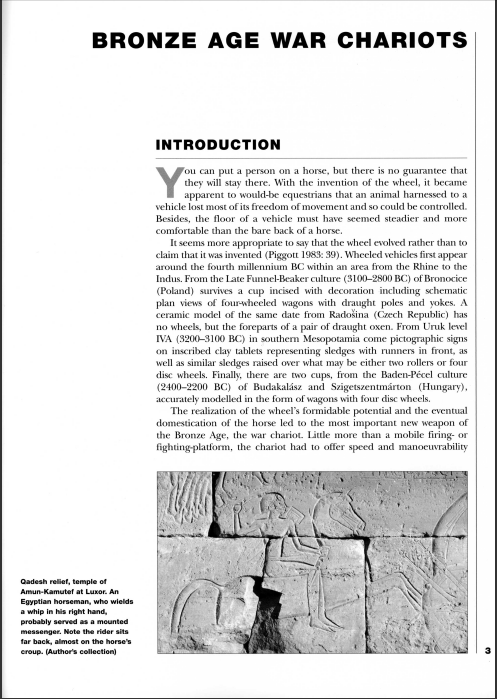
\includegraphics[width=0.5\textwidth]{./chapters/chapter22}}
\end{figure}

\lipsum[1-2]
